% !TEX program = xelatex
\documentclass[12pt,a4paper]{ctexart}

% ---- 页面布局 ----
\usepackage[top=2.5cm, bottom=2.5cm, left=2.8cm, right=2.8cm]{geometry}

% ---- 字体与编码 ----
\usepackage{fontspec}
\setmainfont{Times New Roman}
\setmonofont{Courier New}

% ---- 图表与浮动体 ----
\usepackage{graphicx}
\usepackage{float}
\usepackage{booktabs}
\usepackage{longtable}
\usepackage{multirow}
\usepackage{caption}
\usepackage{subcaption}

% ---- 超链接 ----
\usepackage[colorlinks=true,linkcolor=blue,citecolor=blue,urlcolor=blue,breaklinks=true]{hyperref}
\usepackage{xurl}

% ---- 列表 ----
\usepackage{enumitem}

% ---- 页眉页脚 ----
\usepackage{fancyhdr}
\pagestyle{fancy}
\fancyhf{}
\fancyhead[L]{\small 图像处理与识别大作业}
\fancyhead[R]{\small 基于 YOLOv8 的密集货架商品检测}
\fancyfoot[C]{\thepage}
\renewcommand{\headrulewidth}{0.4pt}

% ---- 代码块 ----
\usepackage{listings}
\lstset{
    basicstyle=\small\ttfamily,
    breaklines=true,
    frame=single,
    aboveskip=6pt,
    belowskip=6pt,
    xleftmargin=1em,
    xrightmargin=1em,
}

% ---- 其他 ----
\usepackage{amsmath}
\usepackage{amssymb}

% ---- 容忍过满盒子 ----
\setlength{\emergencystretch}{1.5em}

% ---- 标题格式定制 ----
\ctexset{
    section/format = \Large\bfseries,
    subsection/format = \large\bfseries,
    subsubsection/format = \normalsize\bfseries,
}

% ==================== 正文 ====================
\begin{document}

% ---------- 封面 ----------
\begin{titlepage}
    \begin{center}
        \vspace*{3cm}

        {\Huge \textbf{基于 YOLOv8 的密集货架商品检测\\[6pt] 微调与性能验证报告}}

        \vspace{2cm}

        {\Large 图像处理与识别 · 课程大作业}

        \vspace{2.5cm}

        {\large
	        \begin{tabular}{rl}
	            \textbf{报告作者} & 刘易函 \\[6pt]
	            \textbf{团队成员} & 刘易函、卓识、陈奕莱、皇甫泊宁 \\[6pt]
	            \textbf{数据集}   & SKU-110K \\[6pt]
	            \textbf{个人基础模型} & YOLOv8n \\[6pt]
	            \textbf{个人实验方向} & 输入尺寸、batch size 与 Mosaic 关闭策略对比
	        \end{tabular}
        }

        \vfill

        {\large \today}
    \end{center}
\end{titlepage}

% ---------- 目录 ----------
\newpage
\tableofcontents
\newpage

% ==================== 摘要 ====================
\section{摘要}

本报告围绕 SKU-110K 密集货架商品检测任务，记录本人刘易函基于 Ultralytics YOLOv8 完成的模型微调、性能验证与外部图片测试。个人实验以 YOLOv8n 为基础模型，在关闭 Mosaic 增强的条件下，分别调整输入尺寸和 batch size，共完成三组微调实验。结果显示，将输入尺寸提高到 800 后，Recall、mAP@0.5 和 mAP@0.5:0.95 均优于另外两组实验；将 batch size 从 32 降至 16 对最终指标影响较小。在团队四组最终结果中，个人 \texttt{finetune2} 的 mAP@0.5:0.95 最高。由于部分对照组缺少完整参数与原始日志，组间结论以描述性比较为主，不作单一变量因果断言。

\medskip
\noindent\textbf{关键词：}YOLOv8；目标检测；SKU-110K；迁移学习；密集小目标；消融实验

% ==================== 项目目标 ====================
\section{项目目标}

本项目需要完成以下工作：

\begin{itemize}[itemsep=2pt]
    \item 选择非 COCO 检测数据集和 YOLOv8 模型变体。
    \item 按 Ultralytics 格式准备数据并记录训练参数。
    \item 完成模型微调，保存日志、权重和可视化结果。
    \item 比较不同实验在逐 epoch 训练过程中的损失和检测指标。
    \item 比较微调前后或不同微调方案的 Precision、Recall、mAP@0.5 和 mAP@0.5:0.95。
    \item 每位成员使用额外 5 张非同源图片进行独立验证。
\end{itemize}

% ==================== 数据集与任务 ====================
\section{数据集与任务}

SKU-110K 是面向超市货架场景的密集目标检测数据集。该数据集中单张图像通常包含大量商品实例，目标尺度较小，遮挡、紧邻和局部重叠现象明显。项目将所有商品统一视为单一检测类别，重点考察模型在密集实例场景中的定位能力。根据项目现有记录，数据集包含 8,219 张训练图片、588 张验证图片和 2,936 张测试图片。

选择该数据集的原因如下：

\begin{itemize}[itemsep=2pt]
    \item 数据集不是 COCO，符合课程要求。
    \item 场景具有明显的密集小目标特征，适合验证输入分辨率和数据增强策略。
    \item 单类别检测减少了类别语义差异的干扰，更适合分析边界框定位能力。
\end{itemize}

训练环境通过 \texttt{SKU-110K.yaml} 指定 \texttt{train}、\texttt{val} 和 \texttt{test} 三个划分，并将类别映射为单一 \texttt{object} 类。图片与标签按 Ultralytics YOLO 检测格式一一对应，每个标签行包含归一化后的 \texttt{class\_id x\_center y\_center width height}。由于数据集体积较大，当前仓库未归档数据本体和 \texttt{SKU-110K.yaml}；复现实验时，需要在原训练环境恢复该配置文件及其指向的数据路径。

% ==================== 模型与方法 ====================
\section{模型与方法}

本人实验使用 \texttt{yolov8n.pt} 作为预训练权重。YOLOv8n 参数量和计算量较小，适合在 vGPU 32GB 环境中进行多组微调对比。三次实验均训练 100 个 epoch，使用相同数据集、随机种子和主要优化参数，并统一关闭 Mosaic 增强。

训练过程记录以下指标：

\begin{itemize}[itemsep=2pt]
    \item 训练损失：Box Loss、Classification Loss、Distribution Focal Loss。
    \item 验证损失：Box Loss、Classification Loss、Distribution Focal Loss。
    \item 检测指标：Precision、Recall、mAP@0.5、mAP@0.5:0.95。
    \item 辅助指标：学习率和累计训练时间。
\end{itemize}

Precision 衡量模型输出检测框中正确检测所占的比例，Recall 衡量真实目标中被成功检出的比例。mAP@0.5 使用 IoU=0.5 作为匹配阈值，mAP@0.5:0.95 则对多个更严格的 IoU 阈值求平均，因此更能反映边界框定位质量。本报告以 mAP@0.5:0.95 作为选择最佳 epoch 的主指标。

% ==================== 实验环境 ====================
\section{实验环境}

\begin{table}[H]
\centering
\caption{实验环境配置}
\label{tab:env}
\begin{tabular}{p{4cm}p{10cm}}
\toprule
\textbf{项目} & \textbf{配置} \\
\midrule
个人训练环境 & Windows Subsystem for Linux 2，vGPU 32GB \\
个人训练软件& Python 3.8+、PyTorch、Ultralytics YOLOv8\\
Baseline 归档环境 & Windows，Python 3.10.20，PyTorch 2.12.0+cu126，Ultralytics 8.4.51 \\
Baseline 归档 GPU & NVIDIA GeForce RTX 4060 Laptop GPU，8188 MiB \\
数据处理      & Pandas、NumPy \\
可视化        & Matplotlib \\
\bottomrule
\end{tabular}
\end{table}

项目通过 \texttt{config.py} 管理训练参数，使用 \texttt{train.py} 启动微调，使用 \texttt{test\_model.py} 执行验证集或测试集评估，使用 \texttt{test\_extra\_images.py} 完成外部图片推理，并通过 \texttt{analyze\_experiments.py} 统一处理多组逐 epoch 日志。个人历史训练未保存 \texttt{pip freeze}、CUDA 和驱动版本，因此本报告不补写无法核实的精确版本；复现实验时应额外保存 \texttt{python --version}、\texttt{pip show torch ultralytics} 和 \texttt{nvidia-smi} 输出。


% ==================== 个人实验设计 ====================
\section{个人实验设计}

\begin{table}[H]
\centering
\caption{三次个人微调实验配置}
\begin{tabular}{cccccc}
\toprule
\textbf{实验} & \textbf{模型} & \textbf{输入尺寸} & \textbf{Batch} & \textbf{Mosaic} & \textbf{Epoch} \\
\midrule
\texttt{finetune1} & YOLOv8n & 640 & 32 & 0.0 & 100 \\
\texttt{finetune2} & YOLOv8n & 800 & 32 & 0.0 & 100 \\
\texttt{finetune3} & YOLOv8n & 640 & 16 & 0.0 & 100 \\
\bottomrule
\end{tabular}
\end{table}

\texttt{finetune1} 作为个人实验基线；\texttt{finetune2} 仅提高输入尺寸，用于观察更高空间分辨率对密集小目标检测的影响；\texttt{finetune3} 仅降低 batch size，用于观察梯度估计规模变化对收敛和泛化的影响。

三次实验的完整参数保存在 \texttt{docs/finetune\_results/*/args.yaml}。共同关键参数包括：\texttt{optimizer=auto}、\texttt{seed=0}、\texttt{deterministic=true}、\texttt{lr0=0.01}、\texttt{lrf=0.01}、\texttt{weight\_decay=0.0005}、\texttt{warmup\_epochs=3}、\texttt{patience=50}、\texttt{amp=true}、\texttt{mixup=0.0} 和 \texttt{copy\_paste=0.0}。\texttt{weights/best.pt} 的检查点元数据包含运行名 \texttt{homeobjects\_n\_no\_mosaic-2}，与 \texttt{finetune2} 的 \texttt{args.yaml} 一致。

\subsection{微调流程与模型选择}

\begin{enumerate}[itemsep=2pt]
    \item 使用 \texttt{yolov8n.pt} 初始化检测模型，并通过 \texttt{SKU-110K.yaml} 加载单类别 SKU-110K 数据。
    \item 按三组配置分别训练 100 个 epoch，每个 epoch 在验证集上记录损失、Precision、Recall 和两项 mAP。
    \item 保存 \texttt{args.yaml}、\texttt{results.csv}、\texttt{results.png} 以及 \texttt{best.pt}、\texttt{last.pt} 等权重；本仓库归档了报告直接使用的参数、CSV 和曲线图。
    \item 以验证集 mAP@0.5:0.95 选择最佳 epoch。三组最佳 epoch 分别为 75、85 和 90，其中 \texttt{finetune2} 在 epoch 85 获得最高值 0.55951。
    \item 将 \texttt{finetune2} 的最佳权重集中保存为 \texttt{weights/best.pt}，再与原始 \texttt{yolov8n.pt} 在同一测试集和同一评估参数下比较。
\end{enumerate}

% ==================== 验证集最终指标 ====================
\section{验证集最终指标}

以下数值来自 \texttt{docs/finetune\_results/} 中各实验 \texttt{results.csv} 的第 100 个 epoch 验证集记录，不等同于独立测试集结果。

\begin{table}[H]
\centering
\caption{三次微调验证集最终指标（epoch 100）}
\small
\setlength{\tabcolsep}{4pt}
\begin{tabular}{lrrrrrrr}
\toprule
\textbf{实验} & \textbf{Precision} & \textbf{Recall} & \textbf{mAP@0.5} & \textbf{mAP@0.5:0.95} & \textbf{最佳 Epoch} & \textbf{最佳 mAP} & \textbf{训练时间} \\
\midrule
\texttt{finetune1} & 0.90961 & 0.83550 & 0.88337 & 0.53988 & 75 & 0.54243 & 97.59 min \\
\texttt{finetune2} & 0.91051 & 0.85209 & 0.89545 & 0.55846 & 85 & 0.55951 & 120.78 min \\
\texttt{finetune3} & 0.90861 & 0.83649 & 0.88425 & 0.54186 & 90 & 0.54324 & 125.11 min \\
\bottomrule
\end{tabular}
\end{table}

与 \texttt{finetune1} 相比，\texttt{finetune2} 的 Recall 提高 0.01659，mAP@0.5 提高 0.01208，mAP@0.5:0.95 提高 0.01858；训练时间增加约 23.8\%。这说明在本实验设置下，更高输入分辨率有助于改善检测效果，但也带来了更高计算开销。

\texttt{finetune3} 与 \texttt{finetune1} 的最终指标非常接近，mAP@0.5:0.95 仅提高 0.00198，但训练时间更长。因此，当前单次实验不足以证明较小 batch size 具有实际优势。

% ==================== 逐 Epoch 变化分析 ====================
\section{逐 Epoch 变化分析}

完整图表由 \texttt{analyze\_experiments.py} 生成，以下列出关键分析图与主要观察结论。

\begin{figure}[H]
    \centering
    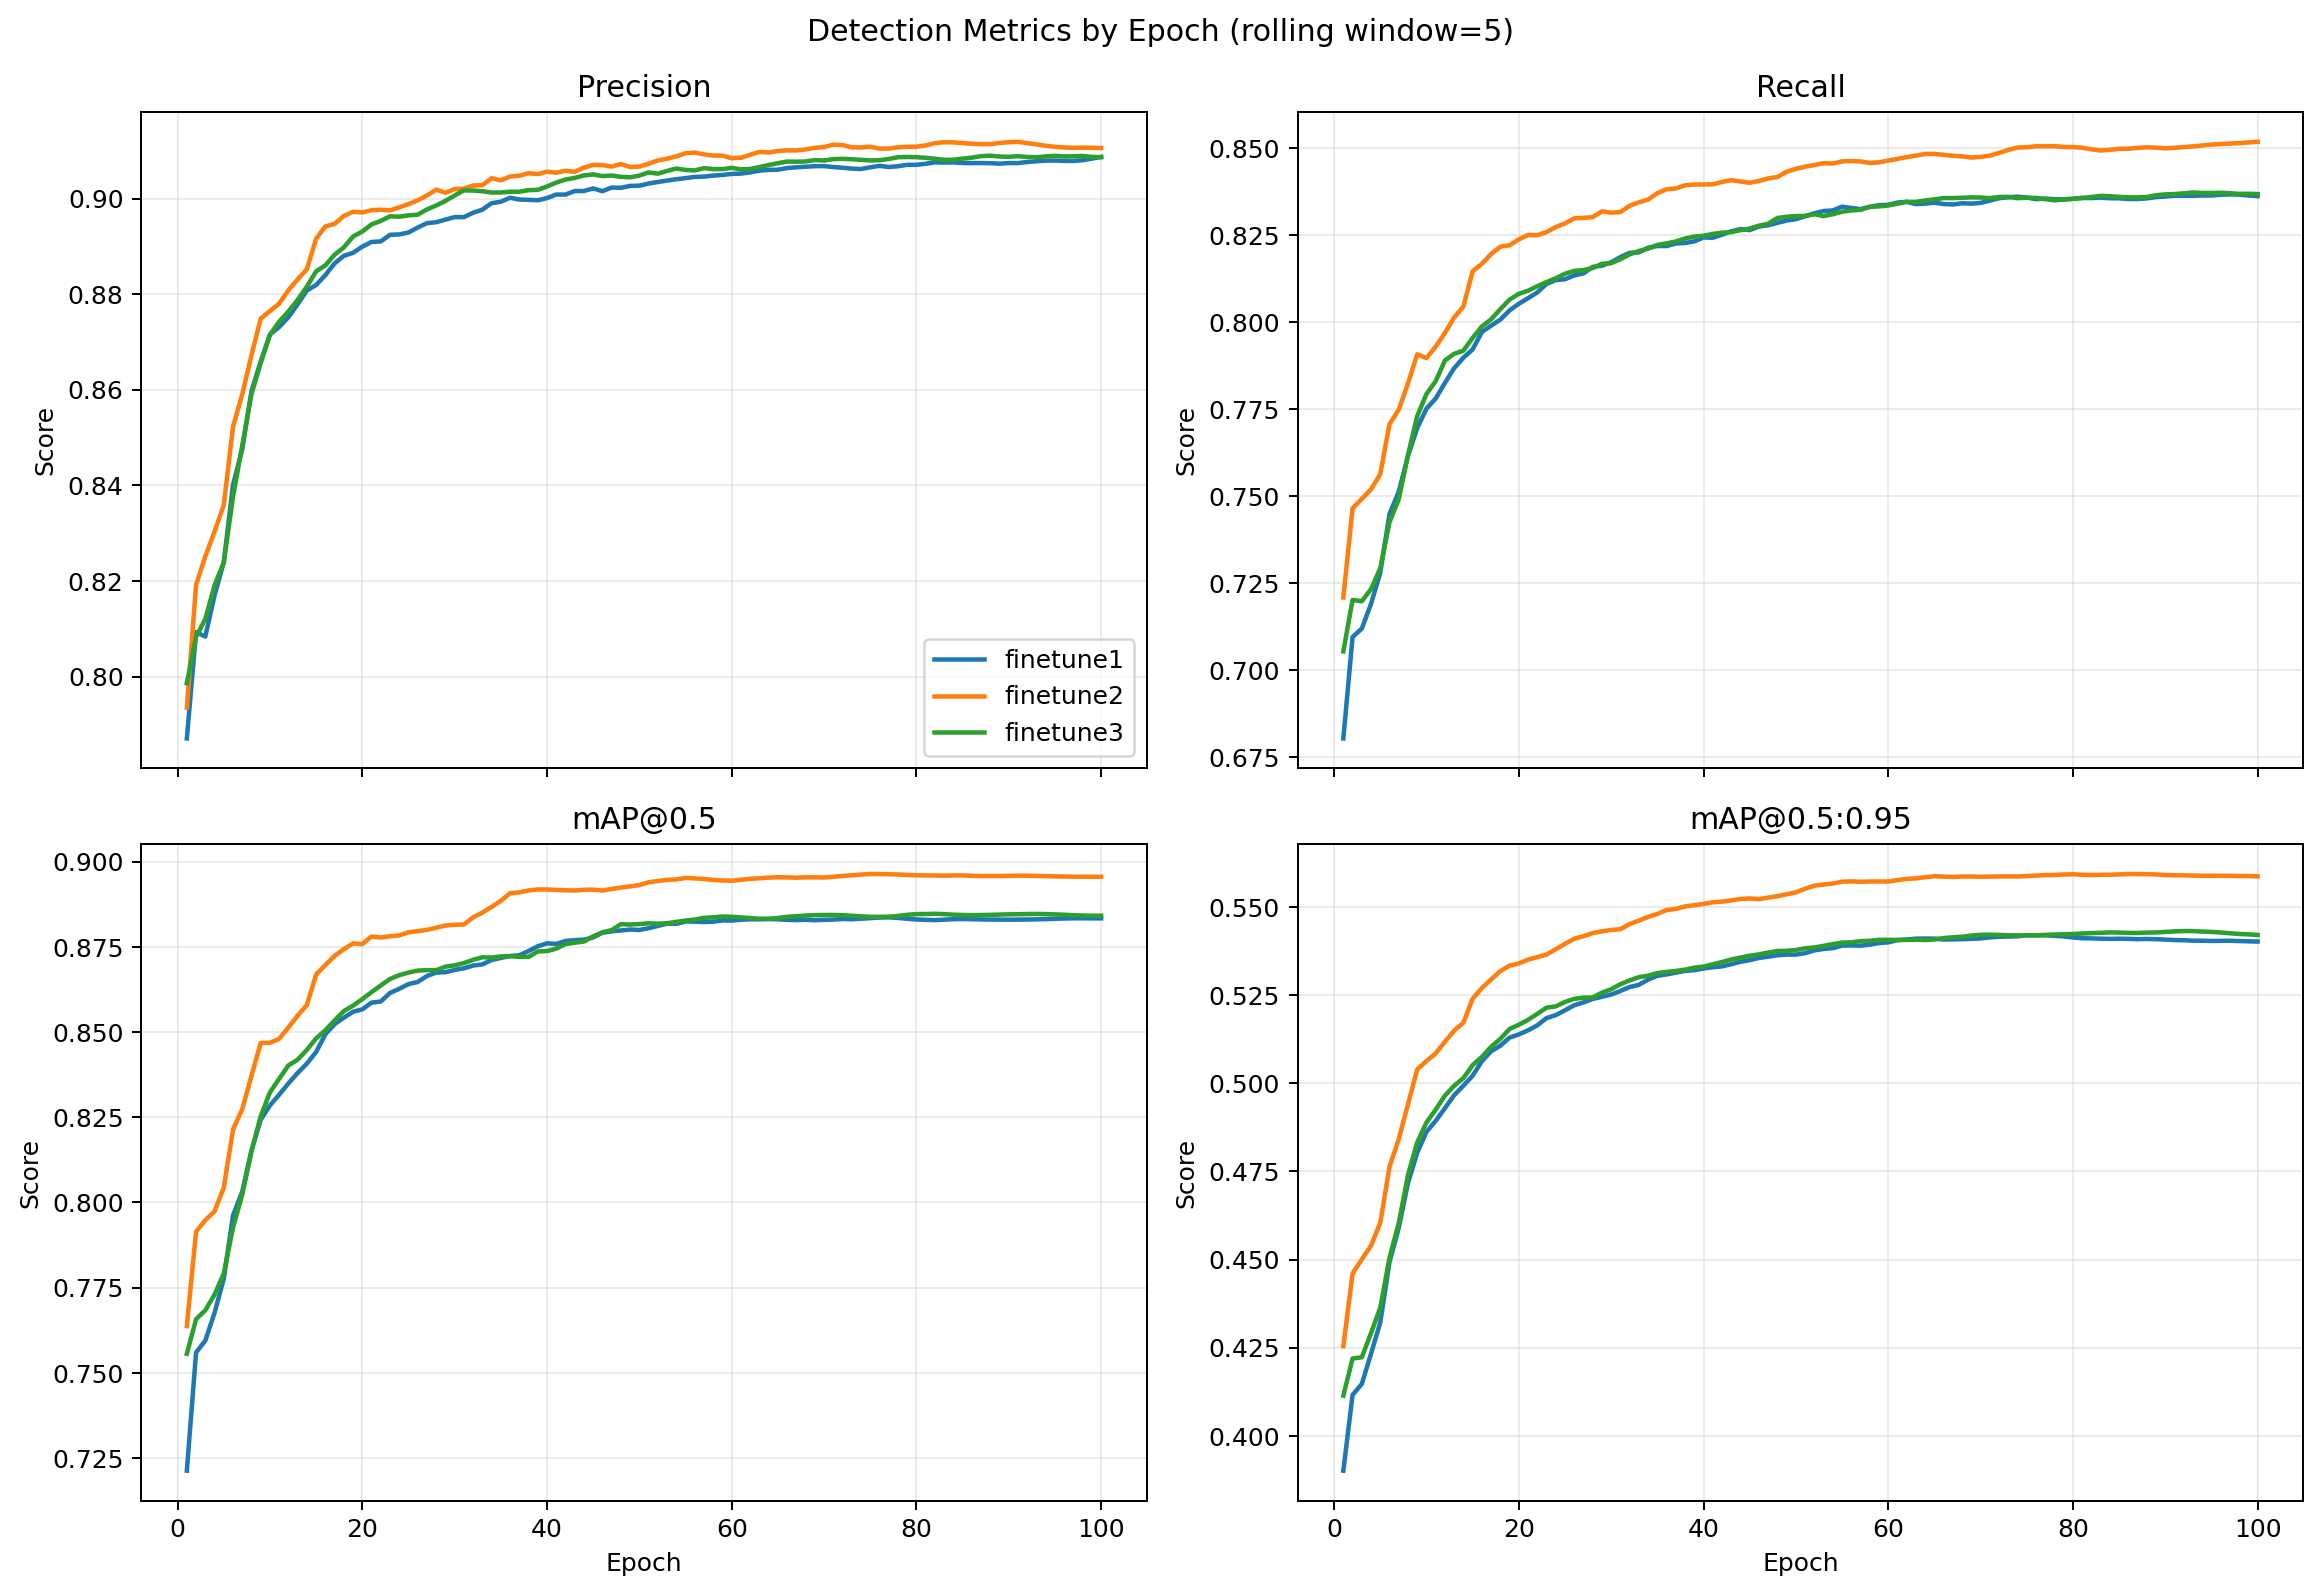
\includegraphics[width=0.88\textwidth]{images/metrics_over_epochs.png}
    \caption{三次微调检测指标变化}
    \label{fig:metrics_over_epochs}
\end{figure}

\begin{figure}[H]
    \centering
    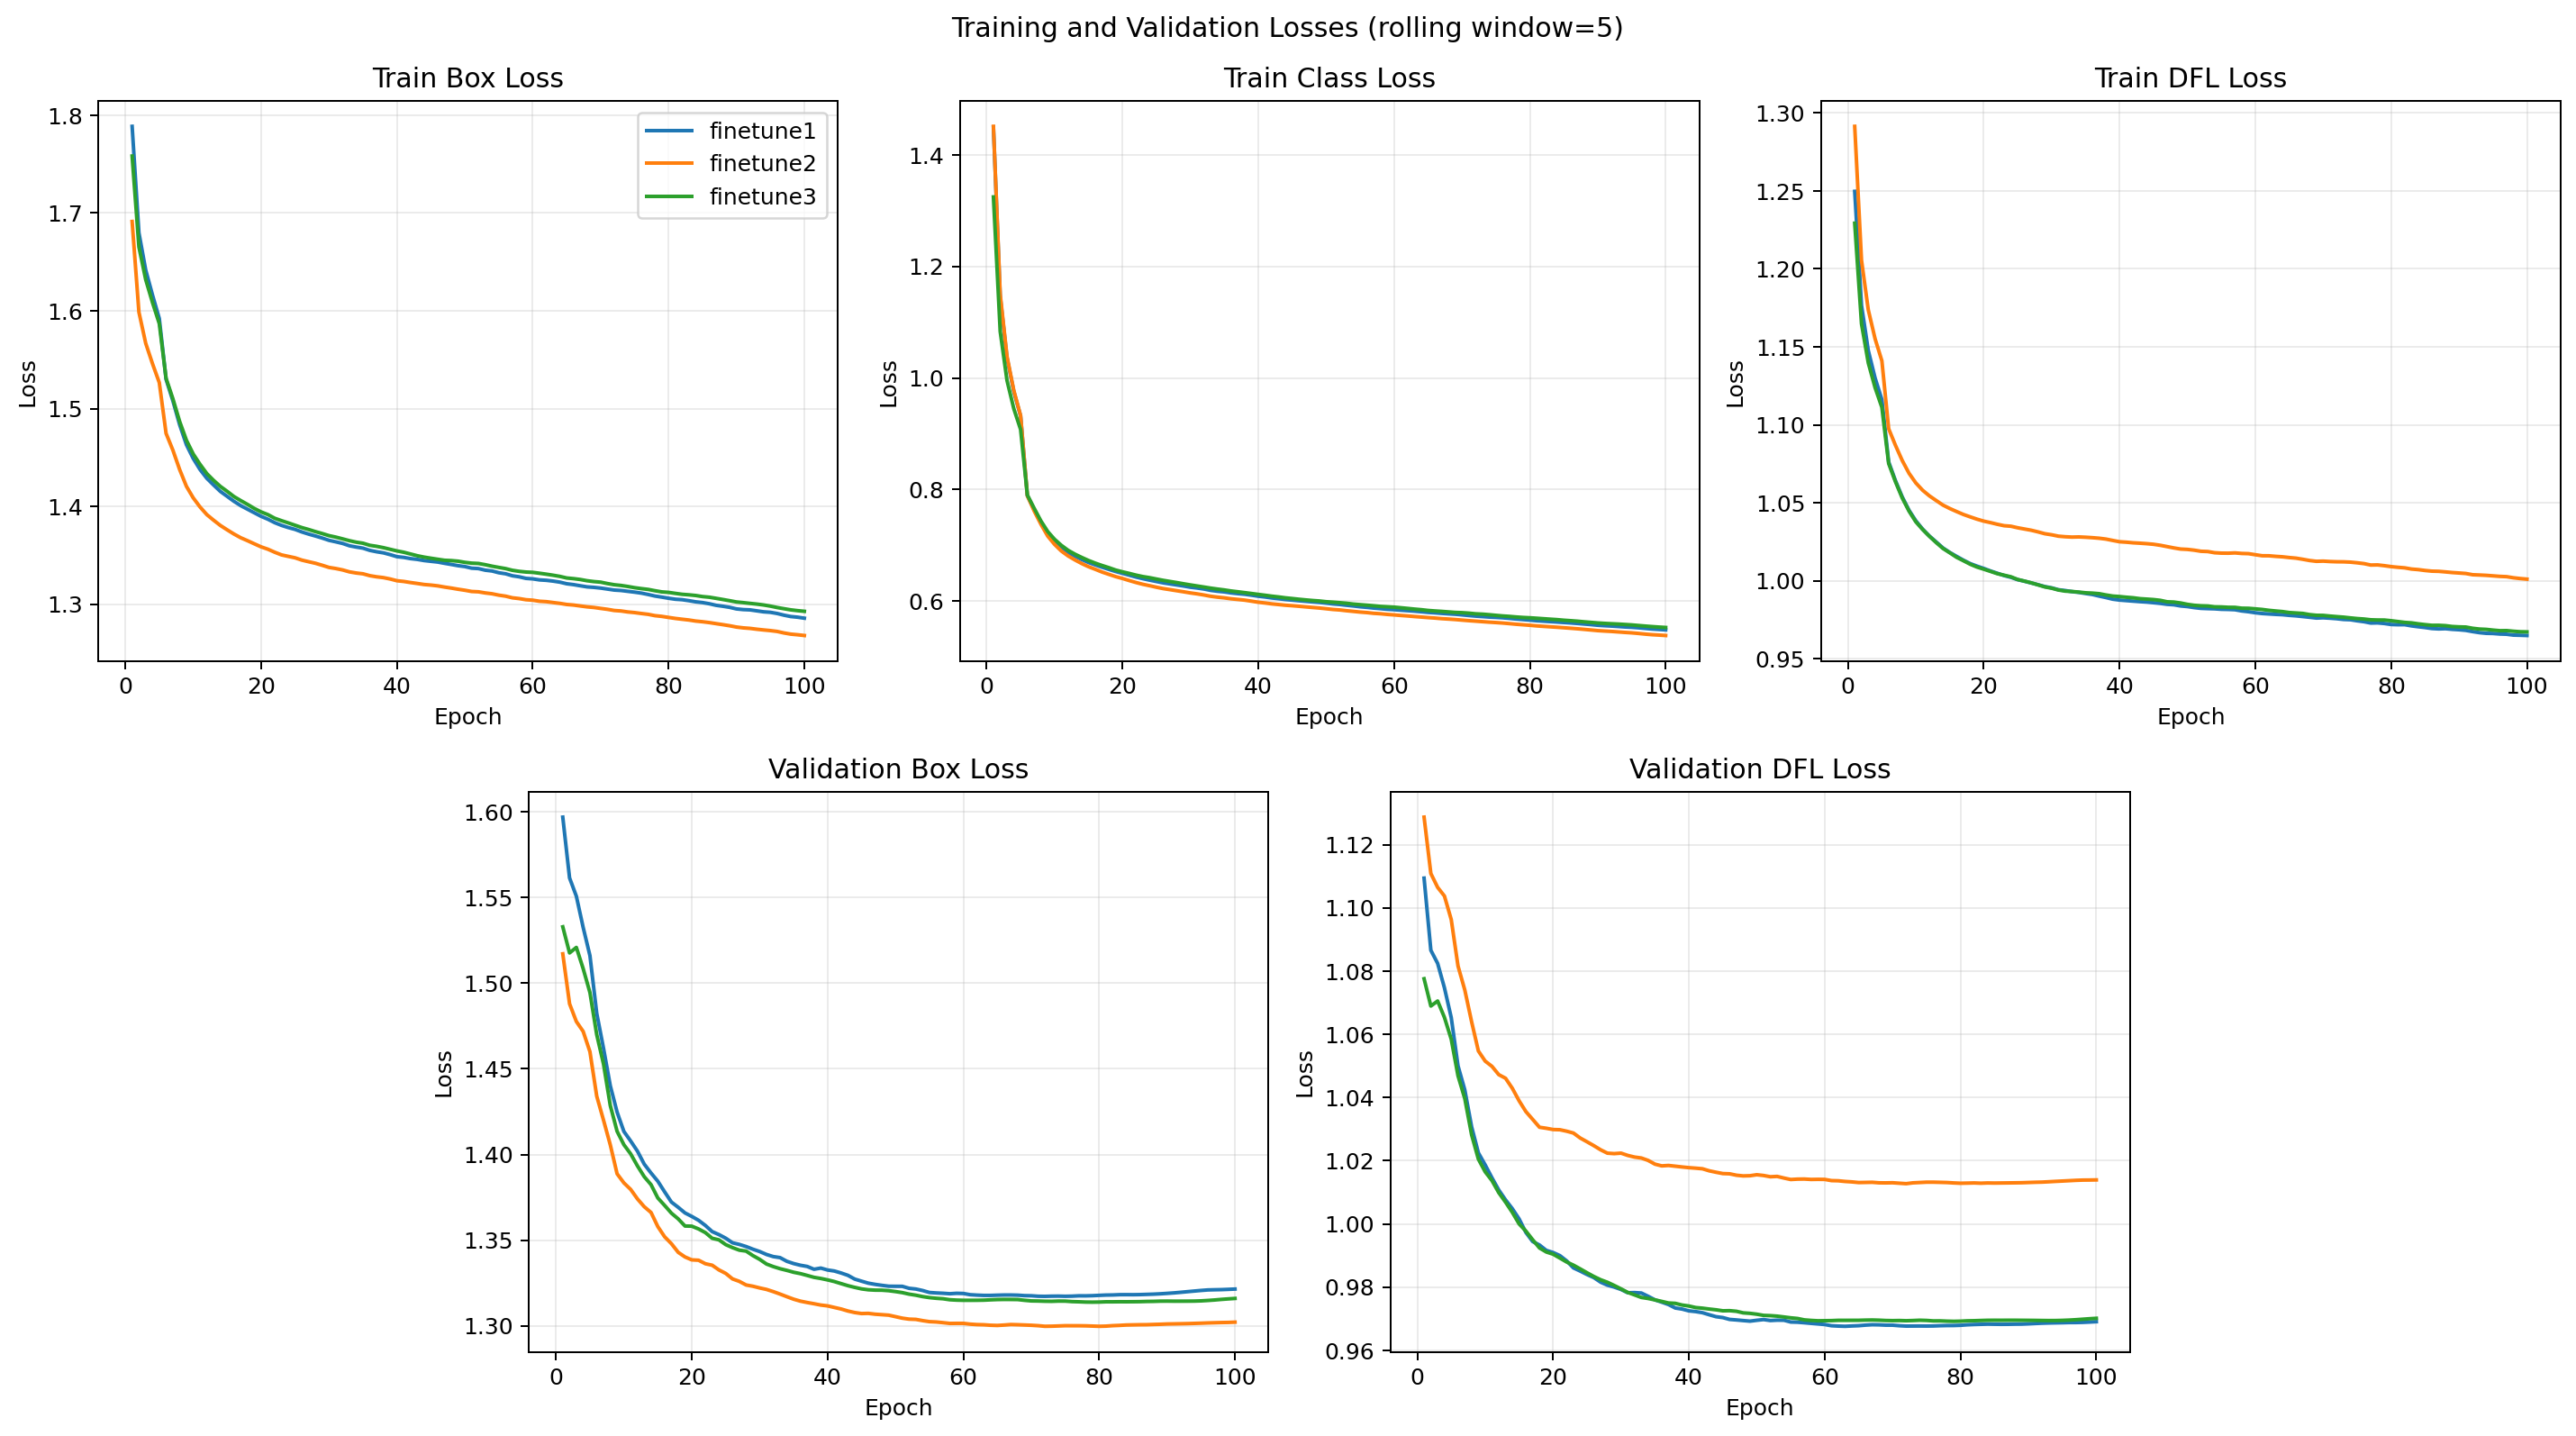
\includegraphics[width=0.88\textwidth]{images/losses_over_epochs.png}
    \caption{三次微调损失变化}
    \label{fig:losses_over_epochs}
\end{figure}

\begin{itemize}[itemsep=2pt]
    \item 三组实验在训练前期检测指标提升较快，后期进入缓慢收敛区间。
    \item \texttt{finetune2} 从训练早期开始就在 Recall 和两项 mAP 上保持较高水平，最终优势并非只来自最后一个 epoch 的随机波动。
    \item \texttt{finetune1} 与 \texttt{finetune3} 的曲线和最终指标接近，需要结合末段标准差判断稳定性，不能仅依据单点数值排序。
    \item 学习率经历预热和后续衰减，检测指标的主要提升集中在训练前中期。
\end{itemize}

三组实验首次达到各自最佳 mAP@0.5:0.95 的 95\% 时，分别位于 epoch 19、15 和 18。\texttt{finetune2} 更早进入有效收敛区间。按 mAP@0.5:0.95 选择最佳 epoch 时，三组实验分别对应 epoch 75、85 和 90，最佳值分别为 0.54243、0.55951 和 0.54324。

\begin{figure}[H]
    \centering
    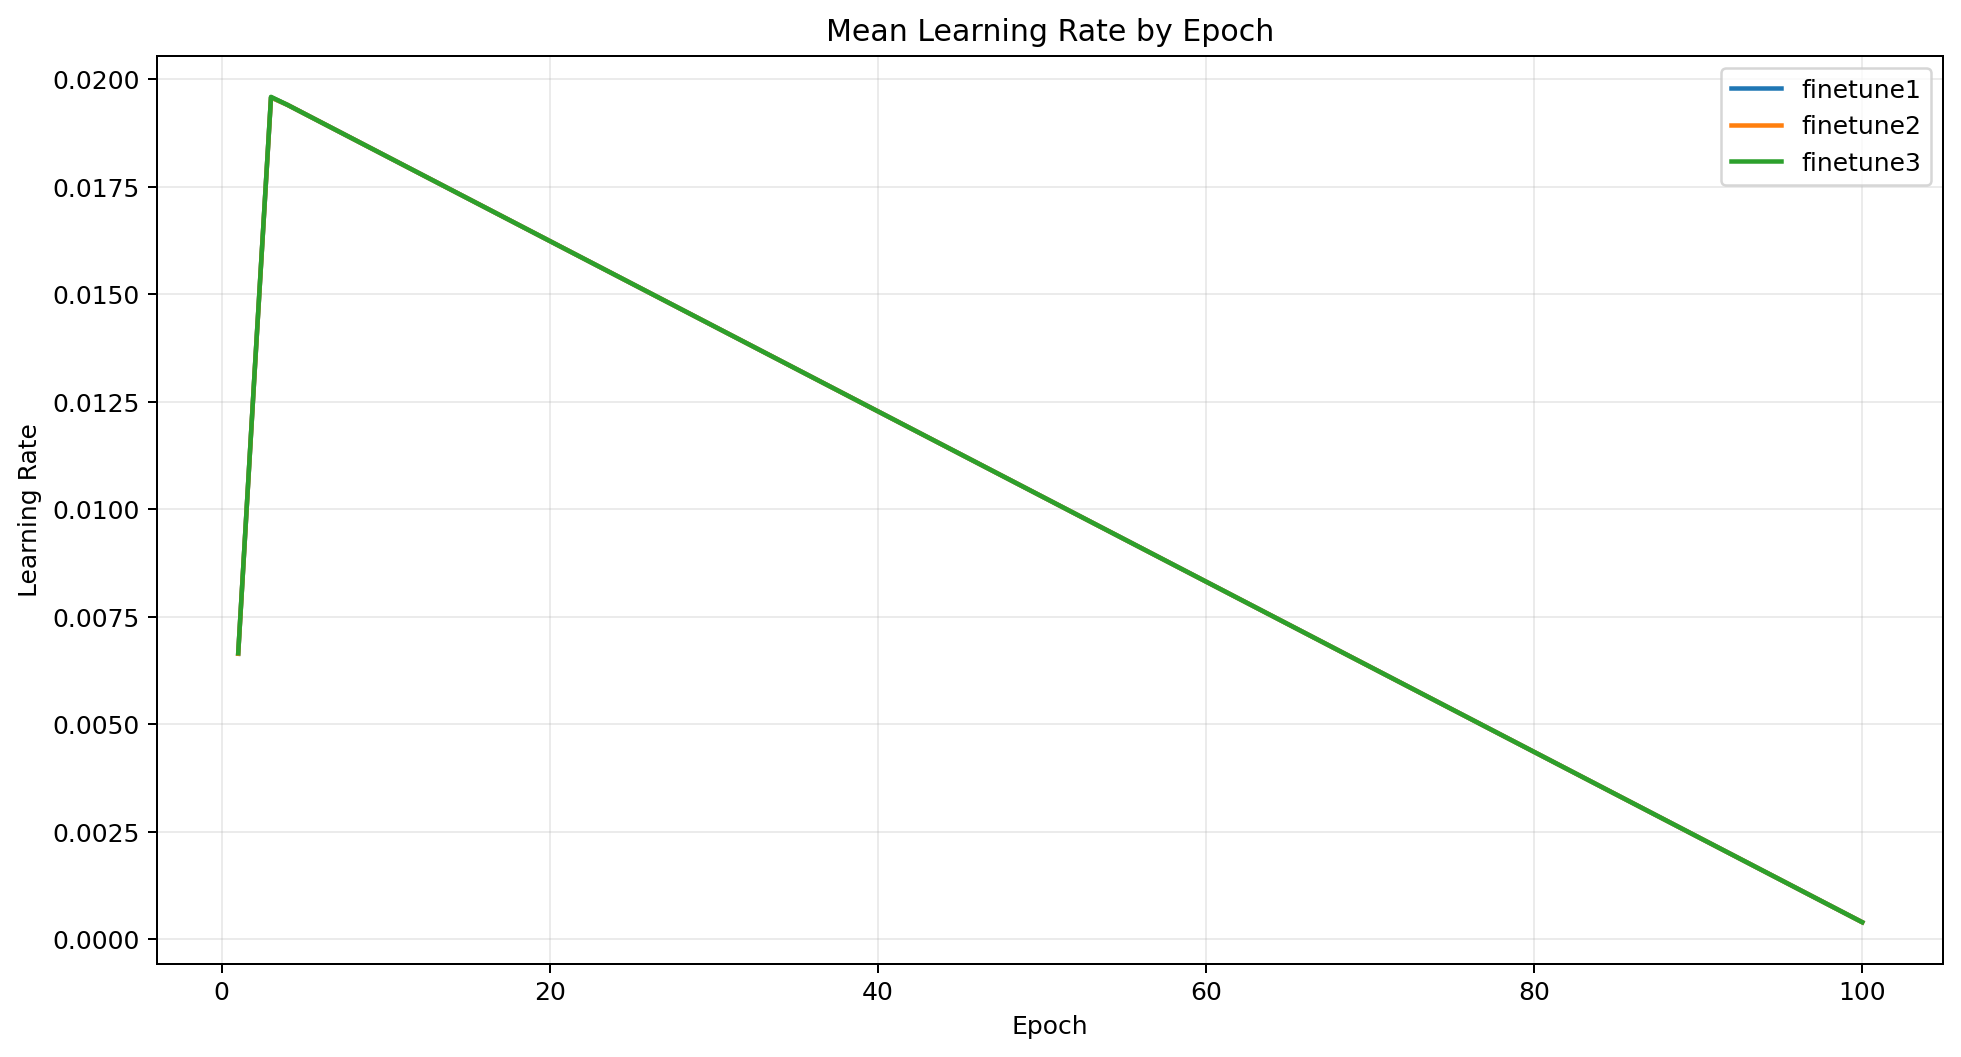
\includegraphics[width=0.85\textwidth]{images/learning_rate_over_epochs.png}
    \caption{三次微调学习率变化}
    \label{fig:lr_over_epochs}
\end{figure}

\begin{figure}[H]
    \centering
    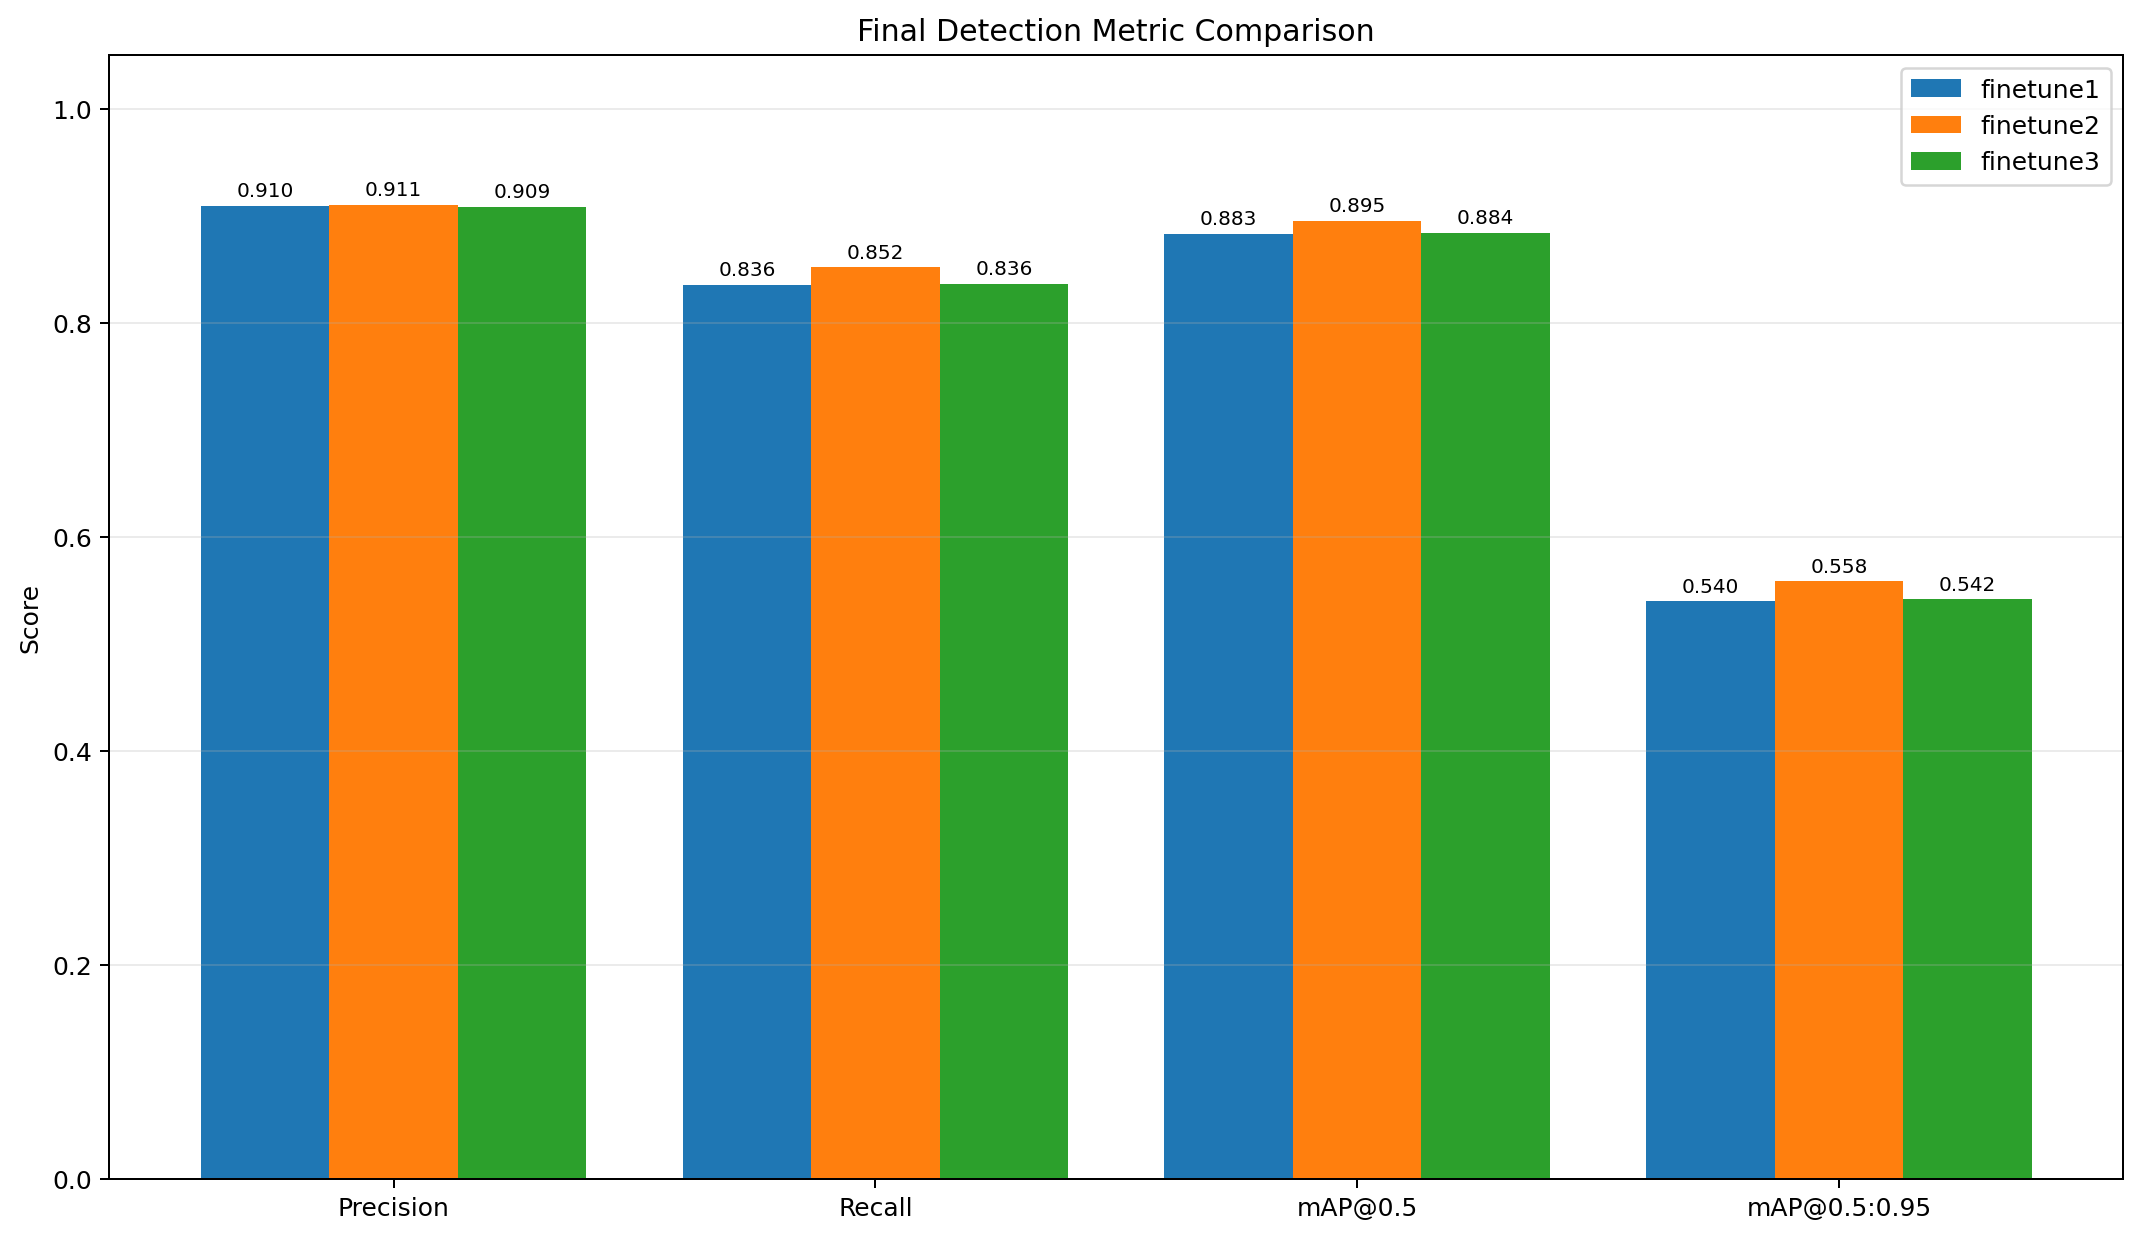
\includegraphics[width=0.85\textwidth]{images/final_metrics_comparison.png}
    \caption{三次微调最终指标对比}
    \label{fig:final_metrics}
\end{figure}

\subsection{数据质量说明}

数据质量检查发现，\texttt{finetune1} 和 \texttt{finetune2} 的 \texttt{val/cls\_loss} 为非有限值 \texttt{inf}。因此，这两组实验不能依据验证分类损失讨论泛化趋势。SKU-110K 为单类别检测任务，但正常情况下该字段仍应为有限数值；本报告仅使用其余有效损失和检测指标，并将该异常保留为训练日志复核事项。

% ==================== 个人实验结论 ====================
\section{个人实验结论}

在当前数据、模型和单次训练条件下，\texttt{finetune2} 是三次个人微调中综合性能最好的方案。提高输入尺寸能够保留更多小目标细节，对密集货架商品定位更有利，主要体现为漏检减少以及严格 IoU 条件下定位质量提高。

输入尺寸提升同时增加训练耗时，最终部署时需要在检测精度、推理速度和显存占用之间权衡。batch size 从 32 降至 16 没有形成明显性能优势，且本次训练耗时更长。由于每种配置仅运行一次，相关结论应表述为当前实验观察，而非普遍规律。

从末 10 个 epoch 的 mAP@0.5:0.95 标准差看，\texttt{finetune1}、\texttt{finetune2} 和 \texttt{finetune3} 分别约为 0.000196、0.000128 和 0.000497。\texttt{finetune2} 后期最稳定，\texttt{finetune3} 波动相对更明显，但三组绝对波动均较小。

% ==================== 微调前后测试集性能比较 ====================
\section{微调前后测试集性能比较}

课程要求的最终比较需要使用 SKU-110K 的 \texttt{test} 划分。评估脚本支持显式指定 \texttt{split=test}，并会将两组指标分别保存为 JSON。为保证比较口径一致，微调前后统一使用 \texttt{imgsz=800}、\texttt{batch=16} 和同一测试集：

\begin{lstlisting}[language=bash]
python test_model.py \
    --pretrained \
    --finetuned \
    --split test \
    --imgsz 800 \
    --batch 16 \
    --output results/test_comparison
\end{lstlisting}

两组模型均使用 SKU-110K 的 \texttt{test} 划分、\texttt{imgsz=800}、\texttt{batch=16} 和 \texttt{device=0}。下表直接采用该文件中的实测结果：

\begin{table}[H]
\centering
\caption{微调前后测试集性能比较}
\begin{tabular}{lrrrr}
\toprule
\textbf{模型} & \textbf{Precision} & \textbf{Recall} & \textbf{mAP@0.5} & \textbf{mAP@0.5:0.95} \\
\midrule
微调前 \texttt{yolov8n.pt} & 0.1211 & 0.0025 & 0.0007 & 0.0003 \\
微调后 \texttt{weights/best.pt} & 0.9117 & 0.8632 & 0.9157 & 0.5736 \\
\midrule
变化量（微调后 $-$ 微调前） & +0.7906 & +0.8607 & +0.9150 & +0.5732 \\
\bottomrule
\end{tabular}
\end{table}

测试结果表明，微调后模型的四项指标均明显提高。其中，Recall 从 0.0025 提高到 0.8632，说明模型对密集货架商品的检出能力得到显著改善；mAP@0.5:0.95 从 0.0003 提高到 0.5736，表明微调不仅增加了检出数量，也改善了多个 IoU 阈值下的综合定位性能。

微调训练使用 \texttt{batch=32}，测试时使用 \texttt{batch=16}。评估 batch 主要影响显存占用和吞吐速度，不改变模型权重；微调前后模型在本次比较中使用相同的评估 batch，因此比较口径一致。测试使用的是 epoch 85 对应的 \texttt{best.pt}，而上一节"验证集最终指标"保留的是第 100 个 epoch 数值，两种口径不能混为一谈。

需要注意，\texttt{yolov8n.pt} 的输出类别是 COCO 80 类，而 SKU-110K 使用单一 \texttt{object} 类，二者标签语义并不完全一致。微调前结果可用于展示迁移学习起点，但不能将差异全部归因于特征提取能力提升。

% ==================== 四组对照试验 ====================
\section{四组对照试验}

\subsection{实验设置}

团队采用四组平行实验，分别考察基线配置、模型容量、数据增强和优化器策略。各组设置如下：

\begin{table}[H]
\centering
\caption{四组平行实验设置}
\small
\begin{tabular}{p{2.8cm}p{1.8cm}p{5.0cm}p{3.8cm}}
\toprule
\textbf{实验组} & \textbf{基础模型} & \textbf{主要设置} & \textbf{实验目的} \\
\midrule
Baseline 调优组 & YOLOv8n & \texttt{imgsz=640}、\texttt{batch=8} & 提供已调参基线 \\
模型容量对比组 & YOLOv8s & \texttt{imgsz=640}、\texttt{batch=8} & 考察增大模型容量的影响 \\
数据增强方案组（个人） & YOLOv8n & \texttt{imgsz=800}、\texttt{batch=32}、\texttt{mosaic=0.0}、100 epoch & 比较关闭 Mosaic 后的个人最佳方案 \\
优化策略调优组 & YOLOv8n & 成员说明为使用 AdamW 优化器 & 考察优化器变化的影响 \\
\bottomrule
\end{tabular}
\end{table}

个人方案使用 \texttt{finetune2} 的 \texttt{weights/best.pt}。需要说明的是，四组在模型、输入尺寸、batch、训练轮数和优化器等方面并未全部统一；个人方案除关闭 Mosaic 外，还将输入尺寸设置为 800。因此，四组结果适合进行最终方案级比较，不能将组间全部差异单独归因于 Mosaic、模型容量或优化器。

\subsection{最终性能汇总}

\begin{table}[H]
\centering
\caption{四组最终性能汇总}
\small
\begin{tabular}{p{3.0cm}rrrrp{5.0cm}}
\toprule
\textbf{实验组} & \textbf{Precision} & \textbf{Recall} & \textbf{mAP@0.5} & \textbf{mAP@0.5:0.95} \\
\midrule
Baseline 调优组 & 0.8960 & 0.8250 & 0.8866 & 0.5360 \\
模型容量对比组 & 0.9110 & 0.8500 & 0.8940 & 0.5590  \\
优化策略调优组 & 0.9110 & 0.8500 & 0.8940 & 0.5590  \\
数据增强方案组 & \textbf{0.9117} & \textbf{0.8632} & \textbf{0.9157} & \textbf{0.5736}  \\
\bottomrule
\end{tabular}
\end{table}

\subsection{结果分析}

\textbf{总体表现。} 以更严格、综合性更强的 mAP@0.5:0.95 作为主要排序指标，个人数据增强方案组排名第一，模型容量对比组与优化策略调优组并列第二，Baseline 调优组排名第四。个人 \texttt{finetune2} 的四项指标均为最高，说明该配置在当前已提供结果中具有最好的综合检测表现。

\textbf{与 Baseline 比较。} \texttt{finetune2} 的 Precision、Recall、mAP@0.5 和 mAP@0.5:0.95 分别提高 0.0157、0.0382、0.0291 和 0.0376。其中 Recall 的提升大于 Precision，表明该方案的主要收益体现在减少密集商品漏检；mAP@0.5:0.95 的提升也说明更严格 IoU 条件下的边界框定位质量有所改善。

\textbf{与模型容量组和优化策略组比较。} 两个对照组当前提供的四项结果完全相同。\texttt{finetune2} 相比它们的 Precision、Recall、mAP@0.5 和 mAP@0.5:0.95 分别高 0.0007、0.0132、0.0217 和 0.0146。三组 Precision 基本相当，但 \texttt{finetune2} 具有更高的 Recall 和 mAP，综合性能略优。

\textbf{模型容量结果。} 模型容量组相对 Baseline 的 Precision、Recall、mAP@0.5 和 mAP@0.5:0.95 分别提高 0.0150、0.0250、0.0074 和 0.0230，表明 YOLOv8s 方案在本次测试中的整体性能高于 Baseline。不过，模型容量组与优化策略组的四项指标完全一致，仍应结合两组原始评估输出确认数据是否分别抄录，避免重复使用同一组结果。

\subsection{比较有效性}

严格横向比较要求四组使用相同的 SKU-110K \texttt{test} 划分，以及一致的 \texttt{imgsz}、置信度阈值、NMS IoU 阈值和模型选择规则。目前个人 \texttt{finetune2} 的结果有 JSON 文件，Baseline 结果有测试终端记录，模型容量组和优化策略组只有人工提供的最终指标。因此，本节能够完成结果汇总和描述性比较，但不能作为严格控制变量实验的最终证据。

Baseline 测试时，SKU-110K 原有 2,936 张图片中的 \texttt{test\_274.jpg} 因文件截断被忽略，最终使用 2,935 张图片和 431,419 个目标实例。成员提供的测试终端记录显示，该次测试环境为 AutoDL 平台服务器，使用 Ultralytics 8.4.51、Python 3.10.20、PyTorch 2.12.0+cu126 和 NVIDIA GeForce RTX 4080 GPU；模型融合后包含 3,005,843 个参数，计算量为 8.1 GFLOPs，单张图片平均推理时间为 1.9 ms。该终端记录与表 \ref{tab:env} 中 Baseline 归档环境的信息来源不同，因此本报告分别保留两处环境信息。

% ==================== 额外五张图片验证 ====================
\section{额外五张图片验证}

本人另选 5 张不属于 SKU-110K 的真实货架图片，使用 \texttt{test\_extra\_images.py} 脚本在统一参数下对预训练模型和微调后模型分别推理。微调后模型使用 \texttt{finetune2}（输入尺寸 800，对应报告"个人实验结论"中的最佳方案）的 \texttt{weights/best.pt}。

\subsection{测试集说明}

\begin{table}[H]
\centering
\caption{额外五张测试图片描述}
\begin{tabular}{lll}
\toprule
\textbf{图片} & \textbf{格式} & \textbf{场景概述} \\
\midrule
\texttt{img1.jpg} & JPEG & 超市谷物货架，标签含西班牙语 \texttt{ARROZ}、\texttt{frijol} \\
\texttt{img2.jpg} & JPEG & 超市冷藏货架，瓶装/盒装饮料密集排列 \\
\texttt{img3.png} & PNG  & 超市货架 \\
\texttt{img4.png} & PNG  & 多层食品货架，罐头、调味品、面包混杂 \\
\texttt{img5.jpg} & JPEG & 超市过道透视场景，源自网络图（含"我图网"水印） \\
\bottomrule
\end{tabular}
\end{table}

5 张图均不来自 SKU-110K 训练集、验证集或测试集，与训练数据无重叠。

\subsection{推理参数}

\texttt{test\_extra\_images.py} 调用的关键参数全部来自 \texttt{config.py}：

\begin{itemize}[itemsep=2pt]
    \item 预训练模型：\texttt{yolov8n.pt}（COCO 80 类）
    \item 微调后模型：\texttt{weights/best.pt}（finetune2）
    \item 输入尺寸：\texttt{config.IMG\_SIZE = 640}
    \item 设备：\texttt{config.DEVICE = 0}（CUDA 可用）
    \item 置信度阈值：\texttt{conf=0.25}
    \item NMS IoU 阈值：\texttt{iou=0.7}
    \item 单图最大检测数：\texttt{max\_det=300}
\end{itemize}

\subsection{检测数对比}

\begin{table}[H]
\centering
\caption{额外图片检测数统计}
\small
\begin{tabular}{p{1.5cm}rp{1.8cm}p{1.8cm}p{5cm}}
\toprule
\textbf{图片} & \textbf{预训练} & \textbf{微调后} & \textbf{置信度区间} & \textbf{主要现象} \\
\midrule
\texttt{img1} & 0 & 48 & 0.26 $\sim$ 0.69 & 预训练模型未输出检测框；微调后在 6 层货架区域输出多个框 \\
\texttt{img2} & 12\footnote{bottle $\times$ 11 + clock $\times$ 1} & 173 & 0.25 $\sim$ 0.78 & 预训练仅识别部分瓶装；把冷藏柜圆形价格牌误识为 clock（0.27）；微调后输出密集候选框 \\
\texttt{img3} & 6\footnote{refrigerator $\times$ 2 + bottle $\times$ 3 + apple $\times$ 1} & 135 & 0.25 $\sim$ 0.77 & 预训练只能命中训练 COCO 时见过的常见类；微调后覆盖货架 \\
\texttt{img4} & 0 & 300 & 0.55 $\sim$ 0.78 & 微调结果达到 \texttt{max\_det=300} 上限；可视化中存在重叠框，底层部分包装未被覆盖 \\
\texttt{img5} & 0 & 144 & 0.25 $\sim$ 0.72 & 含水印的跨来源图片上仍有大量模型响应，准确性需人工标注验证 \\
\midrule
\textbf{总计} & \textbf{18} & \textbf{800} & --- & 微调后输出框更多，但检测数不等同于准确率 \\
\bottomrule
\end{tabular}
\end{table}

\subsection{案例分析}

\textbf{预训练模型的失效模式。} 预训练 YOLOv8n 在 COCO 80 类上预训练，对货架密集商品缺少与 SKU-110K 单类标注相匹配的输出语义。img1、img4、img5 未输出检测框；img2、img3 仅命中若干 \texttt{bottle}、\texttt{refrigerator}、\texttt{apple} 等常见类，且置信度普遍偏低（最高 0.60）。img2 中一处冷藏柜圆形价格牌被误判为 \texttt{clock}（0.27），属于外观相似导致的误检。由于额外图片没有人工标注，此处只能统计零检测，不能称为零召回。

\textbf{微调后模型的候选框分布。} 微调后模型在 5 张外部图上输出了更多候选框，其中 img2 为 173 框、img4 为 300 框、img5 为 144 框。由于这些图片没有人工标注，不能仅凭检测框数量判定性能提升，也不能严格计算过检和漏检。img4 已达到 \texttt{max\_det=300} 上限，实际候选框可能更多。可视化中，中上层罐头和瓶装区域存在重叠框与"框中框"，可能说明极密集场景下 NMS 抑制不足；底层部分包装未被框覆盖，可能与训练分布、域差异、遮挡或推理尺度有关。

\textbf{跨域表现。} img5 是带水印的网络图，与训练集来源不同，模型仍输出 144 个框，说明模型对该场景产生了较强响应。由于没有 ground truth，不能据此直接断言模型具有良好的跨域召回率或鲁棒性。

\textbf{训练分辨率与推理分辨率的差距。} 训练 \texttt{finetune2} 时输入尺寸为 800，本次推理使用 \texttt{config.IMG\_SIZE = 640}，模型在推理时将图像 letterbox 到 640，可能损失一部分小目标细节。这一设置未在脚本层做参数切换，限制了对"高分辨率优势"的更严格验证。

\subsection{可视化对比}

每张图按"预训练 $\to$ 微调后"两行排列。

\begin{figure}[H]
    \centering
    \begin{subfigure}[b]{0.48\textwidth}
        \centering
        \includegraphics[width=\textwidth]{images/img1_pretrained.jpg}
        \caption{预训练}
    \end{subfigure}
    \hfill
    \begin{subfigure}[b]{0.48\textwidth}
        \centering
        \includegraphics[width=\textwidth]{images/img1_finetuned.jpg}
        \caption{微调后}
    \end{subfigure}
    \caption{\texttt{img1} --- 谷物货架}
    \label{fig:img1}
\end{figure}

\begin{figure}[H]
    \centering
    \begin{subfigure}[b]{0.48\textwidth}
        \centering
        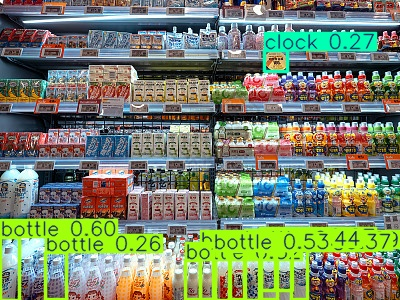
\includegraphics[width=\textwidth]{images/img2_pretrained.jpg}
        \caption{预训练}
    \end{subfigure}
    \hfill
    \begin{subfigure}[b]{0.48\textwidth}
        \centering
        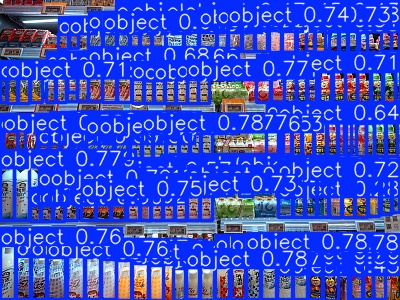
\includegraphics[width=\textwidth]{images/img2_finetuned.jpg}
        \caption{微调后}
    \end{subfigure}
    \caption{\texttt{img2} --- 冷藏货架}
    \label{fig:img2}
\end{figure}

\begin{figure}[H]
    \centering
    \begin{subfigure}[b]{0.48\textwidth}
        \centering
        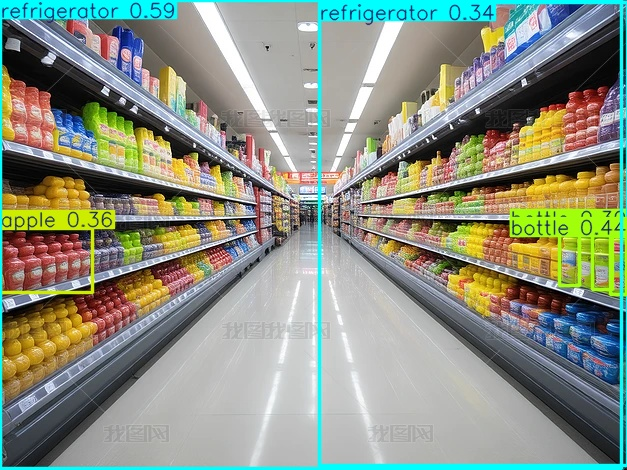
\includegraphics[width=\textwidth]{images/img3_pretrained.jpg}
        \caption{预训练}
    \end{subfigure}
    \hfill
    \begin{subfigure}[b]{0.48\textwidth}
        \centering
        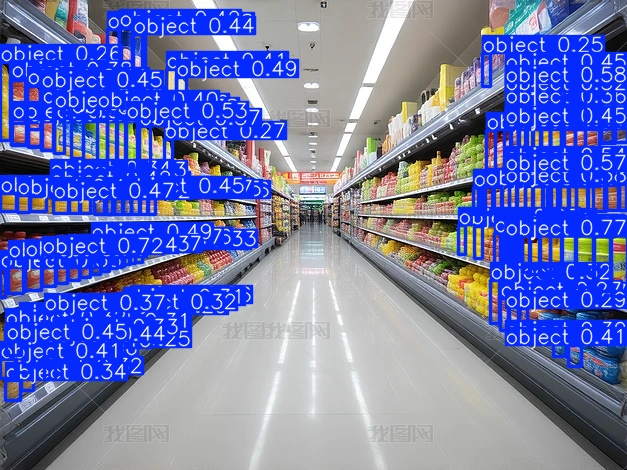
\includegraphics[width=\textwidth]{images/img3_finetuned.jpg}
        \caption{微调后}
    \end{subfigure}
    \caption{\texttt{img3} --- 超市货架}
    \label{fig:img3}
\end{figure}

\begin{figure}[H]
    \centering
    \begin{subfigure}[b]{0.48\textwidth}
        \centering
        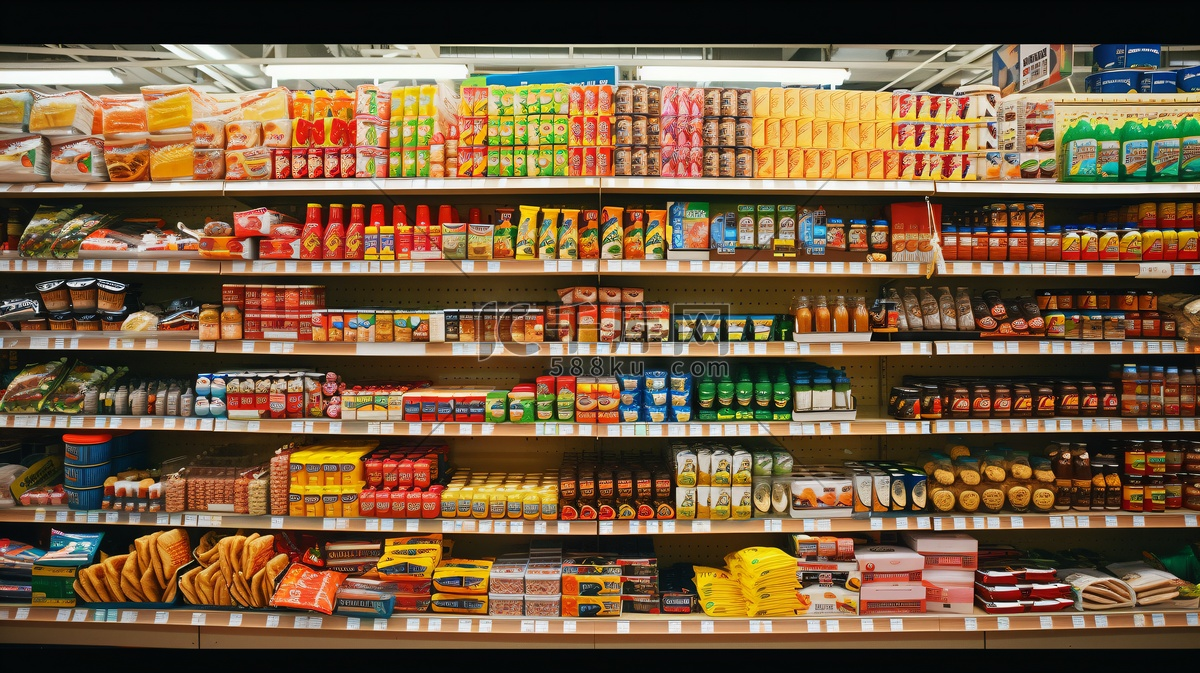
\includegraphics[width=\textwidth]{images/img4_pretrained.jpg}
        \caption{预训练}
    \end{subfigure}
    \hfill
    \begin{subfigure}[b]{0.48\textwidth}
        \centering
        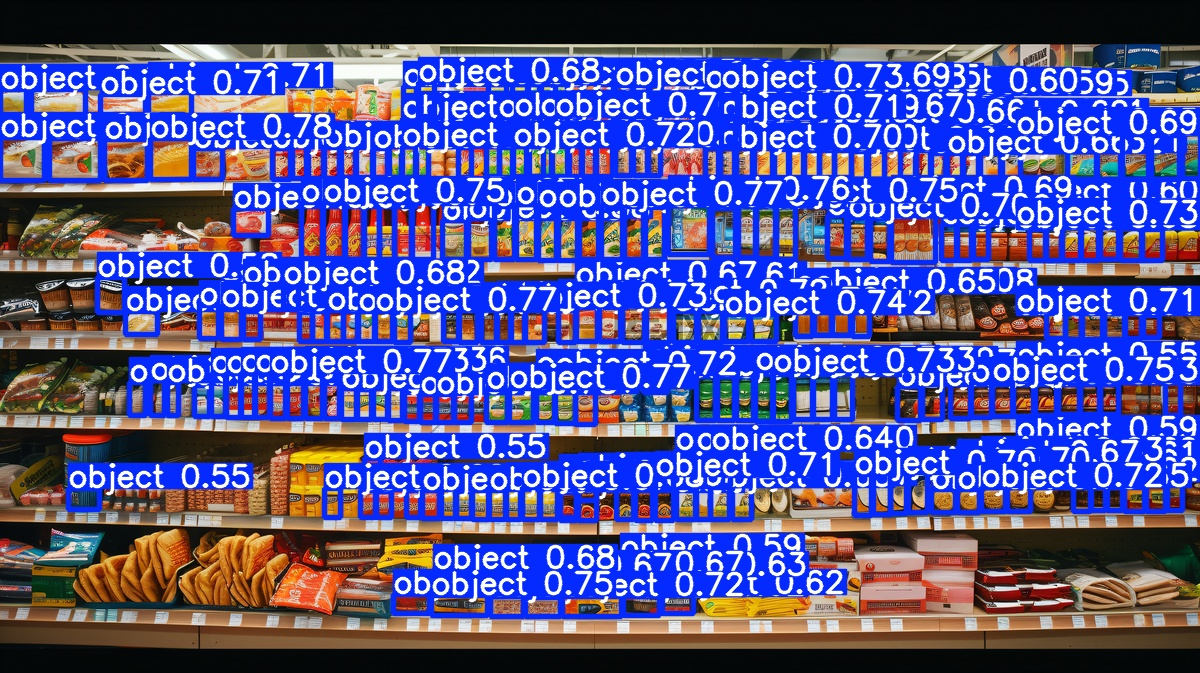
\includegraphics[width=\textwidth]{images/img4_finetuned.jpg}
        \caption{微调后}
    \end{subfigure}
    \caption{\texttt{img4} --- 多层食品货架}
    \label{fig:img4}
\end{figure}

\begin{figure}[H]
    \centering
    \begin{subfigure}[b]{0.48\textwidth}
        \centering
        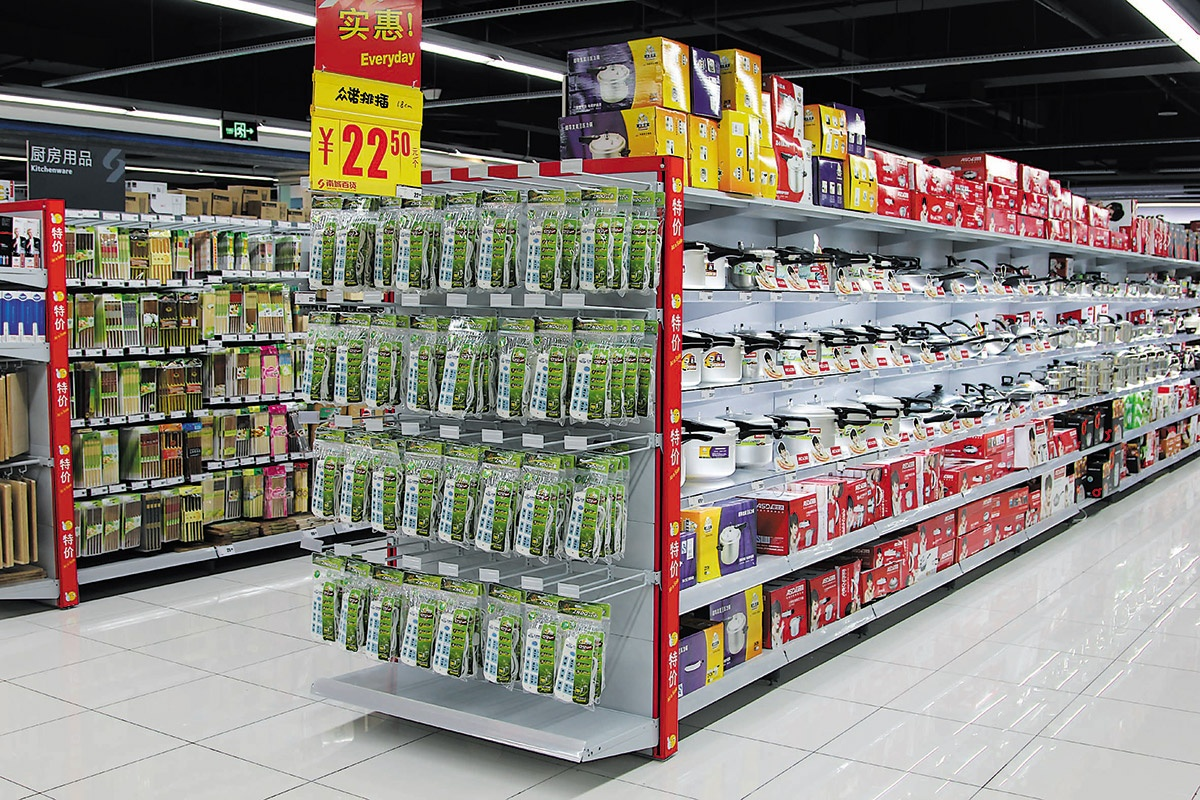
\includegraphics[width=\textwidth]{images/img5_pretrained.jpg}
        \caption{预训练}
    \end{subfigure}
    \hfill
    \begin{subfigure}[b]{0.48\textwidth}
        \centering
        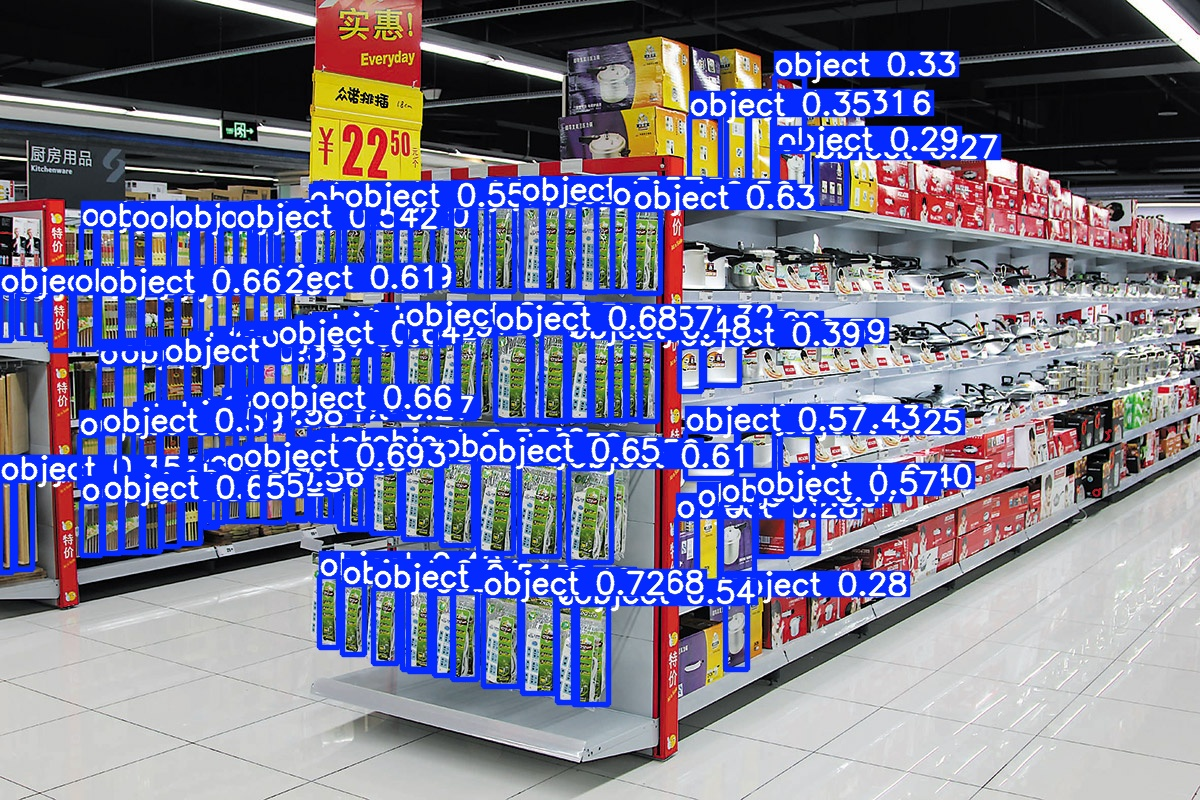
\includegraphics[width=\textwidth]{images/img5_finetuned.jpg}
        \caption{微调后}
    \end{subfigure}
    \caption{\texttt{img5} --- 超市过道}
    \label{fig:img5}
\end{figure}

可视化产物位于 \texttt{test\_images/results/\{pretrained,finetuned\}/} 下，与本节中的图片一一对应。

当前仓库保存了 5 张原图和两组可视化图片，但历史运行没有归档 \texttt{test\_extra\_images.py} 现版本可生成的 \texttt{pretrained\_summary.json} 与 \texttt{finetuned\_summary.json}。报告中的检测数和置信度区间来自已有运行记录；若需完全机器可复核，应在原环境重新运行脚本并保存 JSON 汇总。

% ==================== 局限性 ====================
\section{局限性}

\begin{itemize}[itemsep=2pt]
    \item 每种个人配置仅训练一次，尚未通过多随机种子实验估计方差。
    \item 已完成微调前后模型在 SKU-110K 测试集上的统一评估，但当前只进行了一次测试，尚未通过不同随机种子或重复实验评估结果波动。
    \item 四组对照的训练轮数、输入尺寸和 batch 等设置未完全统一；模型容量组和优化策略组的四项结果完全相同，且缺少原始日志，限制了严格的控制变量分析。
    \item 两组实验的验证分类损失存在 \texttt{inf}，需要检查 Ultralytics 版本、标签缓存和损失记录过程。
    \item 只有 Baseline 保存了推理速度、参数量和 FLOPs，其他组缺少同口径的效率数据，无法完整比较部署成本。
    \item 额外 5 张图片的对比只统计检测数与置信度分布，且预训练 COCO 模型和微调单类别模型的标签语义不同。未做人工 ground truth 标注，因此不能给出可靠的 Precision、Recall 或"提升倍数"。
    \item 5 张图推理使用 \texttt{config.IMG\_SIZE = 640}，未与训练时 finetune2 的 800 输入保持一致，限制了对"高分辨率优势"在外部图上的直接验证。
    \item 当前仓库未包含 SKU-110K 数据本体和 \texttt{SKU-110K.yaml}，跨环境复现前需要恢复数据路径配置。
\end{itemize}

% ==================== 总结 ====================
\section{总结}

本项目已经完成 YOLOv8n 在 SKU-110K 上的三次个人微调、训练日志归档、微调前后测试集性能比较和 5 张外部图片分析。验证集结果中，\texttt{finetune2} 获得最高的 Recall 和 mAP，支持"提高输入分辨率有利于当前密集小目标任务"这一实验观察。测试集上，微调后模型取得 0.9117 Precision、0.8632 Recall、0.9157 mAP@0.5 和 0.5736 mAP@0.5:0.95，在四组最终结果中也排名第一。由于组间训练设置未完全统一、两个对照组结果完全相同且部分原始日志缺失，四组比较目前用于说明方案级表现，不能作为单一变量效果的最终因果结论。

% ==================== 参考资料 ====================
\begin{thebibliography}{9}

\bibitem{sku110k}
Eran Goldman 等. \textit{Precise Detection in Densely Packed Scenes}. CVPR 2019. \\[2pt]
\url{https://openaccess.thecvf.com/content_CVPR_2019/papers/Goldman_Precise_Detection_in_Densely_Packed_Scenes_CVPR_2019_paper.pdf}

\bibitem{ultralytics-train}
Ultralytics. \textit{Model Training with Ultralytics YOLO}. \\[2pt]
\url{https://docs.ultralytics.com/modes/train/}

\bibitem{ultralytics-val}
Ultralytics. \textit{Model Validation with Ultralytics YOLO}. \\[2pt]
\url{https://docs.ultralytics.com/modes/val/}

\end{thebibliography}

\end{document}
